\documentclass{article}
\usepackage[utf8]{inputenc}
\usepackage{graphicx}
\usepackage{tikz}
\usetikzlibrary{shapes.geometric,arrows,shadows, automata}
\usepackage{float}
\usepackage{listings}
\usepackage{caption}

%Tot això hauria d'anar en un pkg, però no sé com és fa
\newcommand*{\assignatura}[1]{\gdef\1assignatura{#1}}
\newcommand*{\grup}[1]{\gdef\3grup{#1}}
\newcommand*{\professorat}[1]{\gdef\4professorat{#1}}
\renewcommand{\title}[1]{\gdef\5title{#1}}
\renewcommand{\author}[1]{\gdef\6author{#1}}
\renewcommand{\date}[1]{\gdef\7date{#1}}
\renewcommand{\maketitle}{ %fa el maketitle de nou
    \begin{titlepage}
        \raggedright{UNIVERSITAT DE LLEIDA \\
            Escola Politècnica Superior \\
            Grau en Enginyeria Informàtica\\
            \1assignatura\\}
            \vspace{5cm}
            \centering\huge{\5title \\}
            \vspace{3cm}
            \large{\6author} \\
            \normalsize{\3grup}
            \vfill
            Professorat : \4professorat \\
            Data : \7date
\end{titlepage}}
%Emplenar a partir d'aquí per a fer el títol : no se com es fa el package
%S'han de renombrar totes, inclús date, si un camp es deixa en blanc no apareix

%\tikzset{
	%Style of nodes. Si poses aquí un estil es pot reutilitzar més facilment
%	pag/.style = {circle, draw=black,
%                           minimum width=0.75cm, font=\ttfamily,
%                           text centered}
%}

\tikzstyle{blue} = [rectangle, rounded corners, minimum width=3cm, text width=3cm,
minimum height=1cm, text centered, draw=black, fill=blue!30]
\tikzstyle{green} = [rectangle, rounded corners, minimum width=3cm, text width=3cm,
minimum height=1cm, text centered, draw=black, fill=green!30]
\tikzstyle{red} = [rectangle, rounded corners, minimum width=3cm, text width=3cm,
minimum height=1cm, text centered, draw=black, fill=red!30]
\tikzstyle{arrow} = [thick,->,>=stealth]

\renewcommand{\figurename}{Figura}
\title{Pràctica 1}
\author{Ian Palacín Aliana}
\date{23 d'Abril de 2019}
\assignatura{Xarxes}
\professorat{ENRIQUE GUITART BARAUT, CARLOS MATEU PIÑOL}
\grup{}

%Comença el document
\begin{document}
\nocite{*}
\maketitle
\thispagestyle{empty}

\newpage
\pagenumbering{roman}
\tableofcontents
\newpage
\pagenumbering{arabic}
\section{Introducció}
Documentació de la pràctica 1 de xarxes. L'objectiu d'aquest projecte és
el de programar una aplicació de xarxes utilitzant el model client-servidor
seguint les pautes d'un protocol de comunicacions. El document està partit
en 5 parts, sent el primer la introducció, seguit d'un diagrama de 
l'estructura del client i el servidor, l'explicació del manteniment 
de la comunicació, el diagrama d'estats UDP i, per últim, consideracions 
a tenir en compte.
\newpage
\section{Diagrames d'estructura}
\subsection{Estructura del client}
\begin{figure}[h]
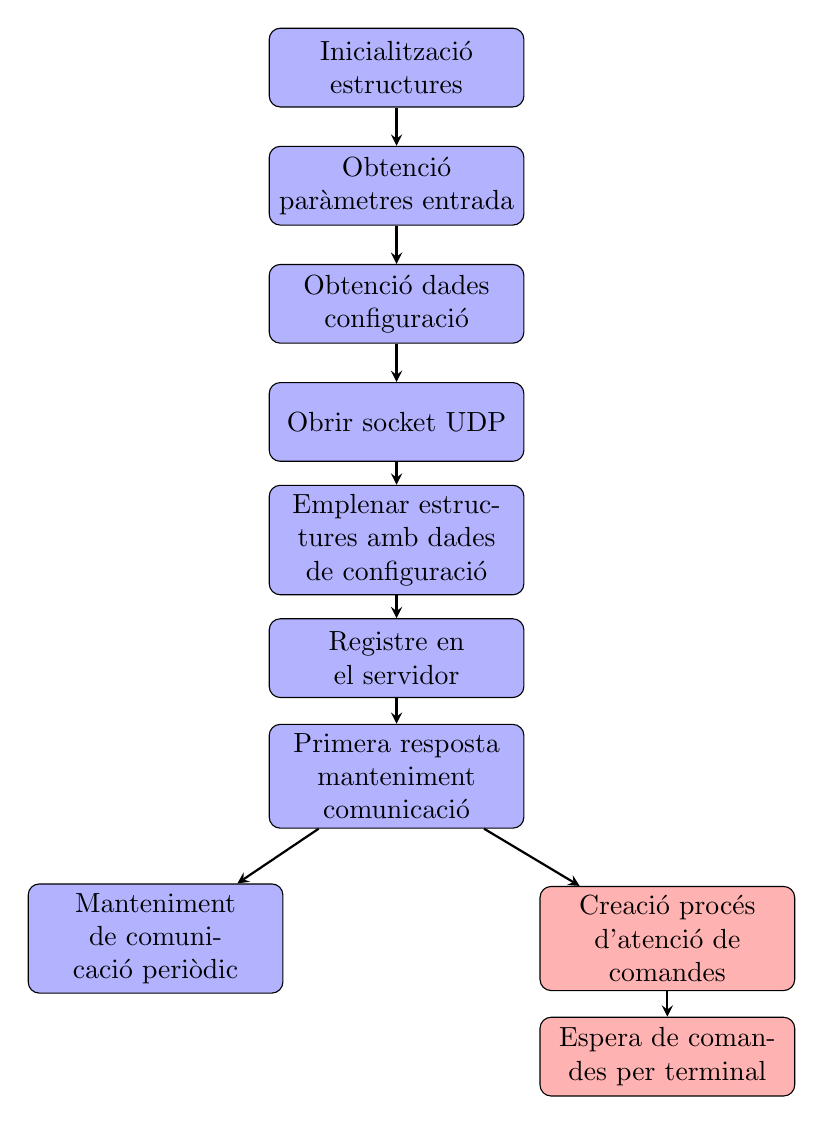
\begin{tikzpicture}[node distance=1.5cm]
\node (1)[blue]{Inicialització estructures};
\node (2)[blue, below of=1]{Obtenció paràmetres entrada};
\node (3)[blue, below of=2]{Obtenció dades configuració};
\node (4)[blue, below of=3]{Obrir socket UDP};
\node (5)[blue, below of=4]{Emplenar estructures amb dades de configuració};
\node (6)[blue, below of=5]{Registre en el servidor};
\node (7)[blue, below of=6]{Primera resposta manteniment comunicació};
\node (8)[blue, below left of=7,xshift=-2cm, yshift=-1cm]{Manteniment de comunicació periòdic};
\node (9)[red, right of= 8, xshift=5cm]{Creació procés d'atenció de comandes};
\node (10)[red, below of=9]{Espera de comandes per terminal};

\draw [arrow](1) -- (2);
\draw [arrow](2) -- (3);
\draw [arrow](3) -- (4);
\draw [arrow](4) -- (5);
\draw [arrow](5) -- (6);
\draw [arrow](6) -- (7);
\draw [arrow](7) -- (8);
\draw [arrow](7) -- (9);
\draw [arrow](9) -- (10);
\end{tikzpicture}
\caption{Diagrama de blocs de l'estructura del client}
\end{figure}
\newpage
\subsection{Estructura del servidor}
\begin{figure}[h]
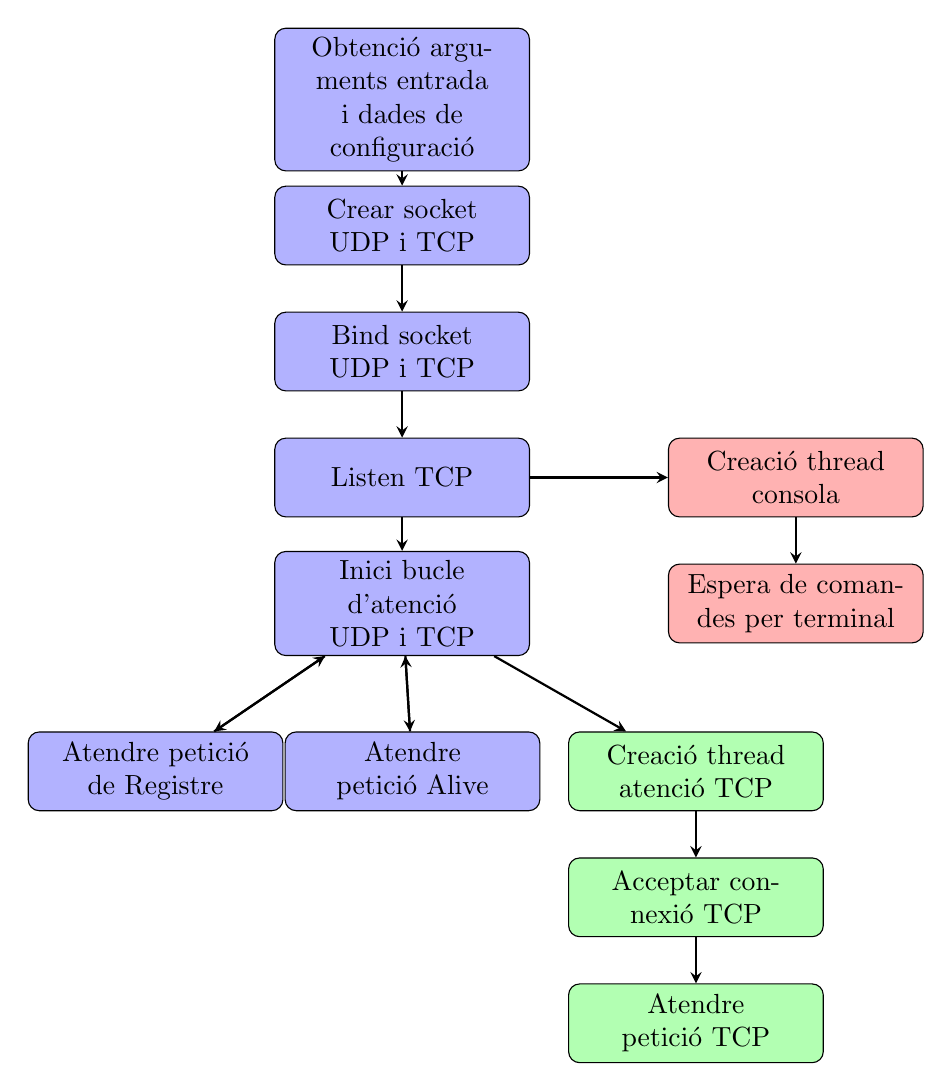
\begin{tikzpicture}[node distance=1.6cm]
\node (1)[blue, xshift=2cm]{Obtenció arguments entrada i dades de configuració};
\node (2)[blue, below of=1]{Crear socket UDP i TCP};
\node (3)[blue, below of=2]{Bind socket UDP i TCP};
\node (4)[blue, below of=3]{Listen TCP};
\node (5)[blue, below of=4]{Inici bucle d'atenció UDP i TCP};
\node (6)[blue, below left of=5, xshift=-2cm, yshift=-1cm]{Atendre petició de Registre};
\node (7)[blue, below right of=5, xshift=-1cm, yshift=-1cm]{Atendre petició Alive};
\node (8)[green, right of=7, xshift=2cm]{Creació thread atenció TCP};
\node (9)[green, below of=8]{Acceptar connexió TCP};
\node (10)[green, below of=9]{Atendre petició TCP};
\node (11)[red, right of=4, xshift=34mm]{Creació thread consola};
\node (12)[red, below of=11]{Espera de comandes per terminal};

\draw [arrow](1) -- (2);
\draw [arrow](2) -- (3);
\draw [arrow](3) -- (4);
\draw [arrow](4) -- (5);
\draw [arrow](5) -- (6);
\draw [arrow](5) -- (7);
\draw [arrow](5) -- (8);
\draw [arrow](8) -- (9);
\draw [arrow](9) -- (10);
\draw [arrow](4) -- (11);
\draw [arrow](11) -- (12);
\draw [arrow](7) -- (5);
\draw [arrow](6) -- (5);
\end{tikzpicture}
\caption{Diagrama de blocs de l'estructura del servidor}
\end{figure}
\newpage

\section{Manteniment de comunicació}
\subsection{Manteniment de comunicació del client}

Una vegada el client s'ha registrat, passa a la fase de manteniment
de comunicació amb el servidor. Per entendre l'estratègia emprada
primer s'han d'introduir unes variables importants. La primera
és \textbf{intent}, és el comptador d'intents d'alive. Variable de tipus 
enter que s'inicialitzarà a
0 i anirà canviant de valor en funció dels paquets que li arribin (o li
deixin d'arribar). \textbf{Intent} ajudarà a sortir en el moment adient
del bucle principal d'enviament d'ALIVE\textunderscore INF com, per 
exemple, quan es rep un ALIVE\textunderscore REJ (es veuran tots els 
altres casos més endavant).\\

La segona variable a mencionar és \textbf{first}, variable de tipus enter
però que funciona com una booleana. Aquesta variable serveix per saber si
ja s'ha rebut el primer ALIVE\textunderscore REQ. S'inicialitza a 1 i 
en recepció de la primera confirmació d'alive passa a 0, nombre en 
el qual es quedarà durant tota la resta de procés de manteniment 
de comunicació.\\

El procés de manteniment de comunicació consta d'un bucle principal, 
que s'executarà mentres \textbf{intent} sigui menor a \textbf{u}, 
el nombre màxim de temps d'alive permesos sense rebre confirmació.  
A cada iteració del bucle s'enviarà una petició d'alive i s'esperarà
un temps d'alive (r). Si després de l'espera no s'ha rebut resposta
del servidor, s'incrementarà \textbf{intent} i es tornarà a dalt del
bucle. Si després de l'espera s'ha rebut resposta, aquesta es tractarà
de la següent manera:
\begin{itemize}
\item Si la resposta és un ALIVE\textunderscore ACK 
del servidor corresponent, es ficarà el comptador d'intents a 0 de 
nou, d'aquesta manera es podran tornar a permetre \textbf{r} 
ALIVE\textunderscore INF sense resposta. Si \textbf{first} val 1 voldrà 
dir que és la primera confirmació d'alive i, per tant
, el client canviarà d'estat registrat a alive. En aquest moment és
també quan es crea el procés de consola. 
\item La recepció d'un ALIVE\textunderscore REJ del servidor corresponent
es considerarà com suplantació d'identitat i es ficarà el comptador 
d'intents a \textbf{u} (nombre màxim d'intents sense confirmació 
permesos), d'aquesta manera acabarà el bucle i la fase d'alive, tornant 
a la fase de registre
\item En qualsevol altre cas, que és la recepció d'un paquet no autoritzat
o d'un paquet de tipus ALIVE\textunderscore NACK es considerarà com no haver 
rebut resposta del servidor, i simplement s'incrementarà el comptador d'intents
\end{itemize}
Utilitzant aquest sistema s'aconsegueix el manteniment de connexió  corresponent 
amb el servidor per part del client.
\newpage 

\subsection{Manteniment de comunicació del servidor}

En la part del servidor, cada client que ha superat la fase de registre, té un camp
anomenat TTL que fa referència al temps (en temps d'alives) que li queda fins a ser 
desconnectat. Quan aquest camp arriba a 0, es considera que s'ha perdut connexió amb
el client i passa a l'estat DISCONNECTED.\\

Perquè a cada temps d'alive es puguin actualitzar els TTL dels clients i a l'hora
atendre totes les altres peticions del servidor, s'utilitzen threads concurrents. El
programa principal és el que atendrà les peticions TCP i UDP. Cada vegada que es rebi
un ALIVE\textunderscore INF correcte es crearà un thread que sumarà \textbf{k} (3) al
camp TTL del client que ha enviat la petició. Acte seguit a cada temps d'alive li anirà
restant 1, si s'arriba a 0 vol dir que no s'ha rebut cap ALIVE\textunderscore INF en el
transcurs d'aquests 3 temps d'alive. Això és degut al fet que si s'hagués rebut una altra 
petició d'alive del mateix client, s'hauria creat un altre thread, que li hauria 
sumat k (3) TTLs més.\\

Aquest sistema és possible gràcies al fet que les variables 
globals estan compartides entre
threads d'un mateix procés; i la informació dels clients (on s'actualitzen els
TTLS) estan en una llista de diccionaris de forma global. Una vegada entés 
el sistema de TTL, es pot explicar de forma més ordenada el procés sencer 
de manteniment de comunicació.\\

Una vegada el servidor ha rebut la petició de registre correcta i l'ha respost 
de forma adequada, el servidor ha de rebre un alive en menys de 2 temps d'alive. 
És per això que el servidor només acabar la fase de registre del client crea 
un thread dels comentats anteriorment, però en comptes de sumar 3 TTLs, li suma 2.\\
Mentre el thread secundari va restant els temps d'alive, el thread principal va
atenent les peticions que li arriben pels canals UDP i TCP. Atén els 
ALIVE\textunderscore INF de la següent forma:

\begin{itemize}

\item Quan rep un ALIVE\textunderscore INF d'un client, mira si aquest 
està autoritzat, en l'estat correcte, i si el nombre aleatori i IP 
concorden amb el client registrat. Si tot és correcte se li enviarà 
un ALIVE\textunderscore ACK i es crearà un thread de descompte de TTL 
de 3 temps d'alive. Si l'estat del client era REGISTERED, aquest
passarà a ALIVE.\\

\item Si la petició prové d'un client no autoritzat o que no està en els 
estats REGISTERED o ALIVE, se li enviarà un ALIVE\textunderscore REJ 
informant-lo del motiu.

\item Si la IP o el nombre aleatori del client no concorden se li enviarà
un ALIVE\textunderscore NACK informant-lo del motiu.
\end{itemize}
Amb aquest sistema de TTLs s'aconsegueix mantenir la comunicació corresponent
amb els clients necessaris de forma concurrent per part del servidor.

\section{Diagrama d'estats UDP}
\begin{figure}[h]
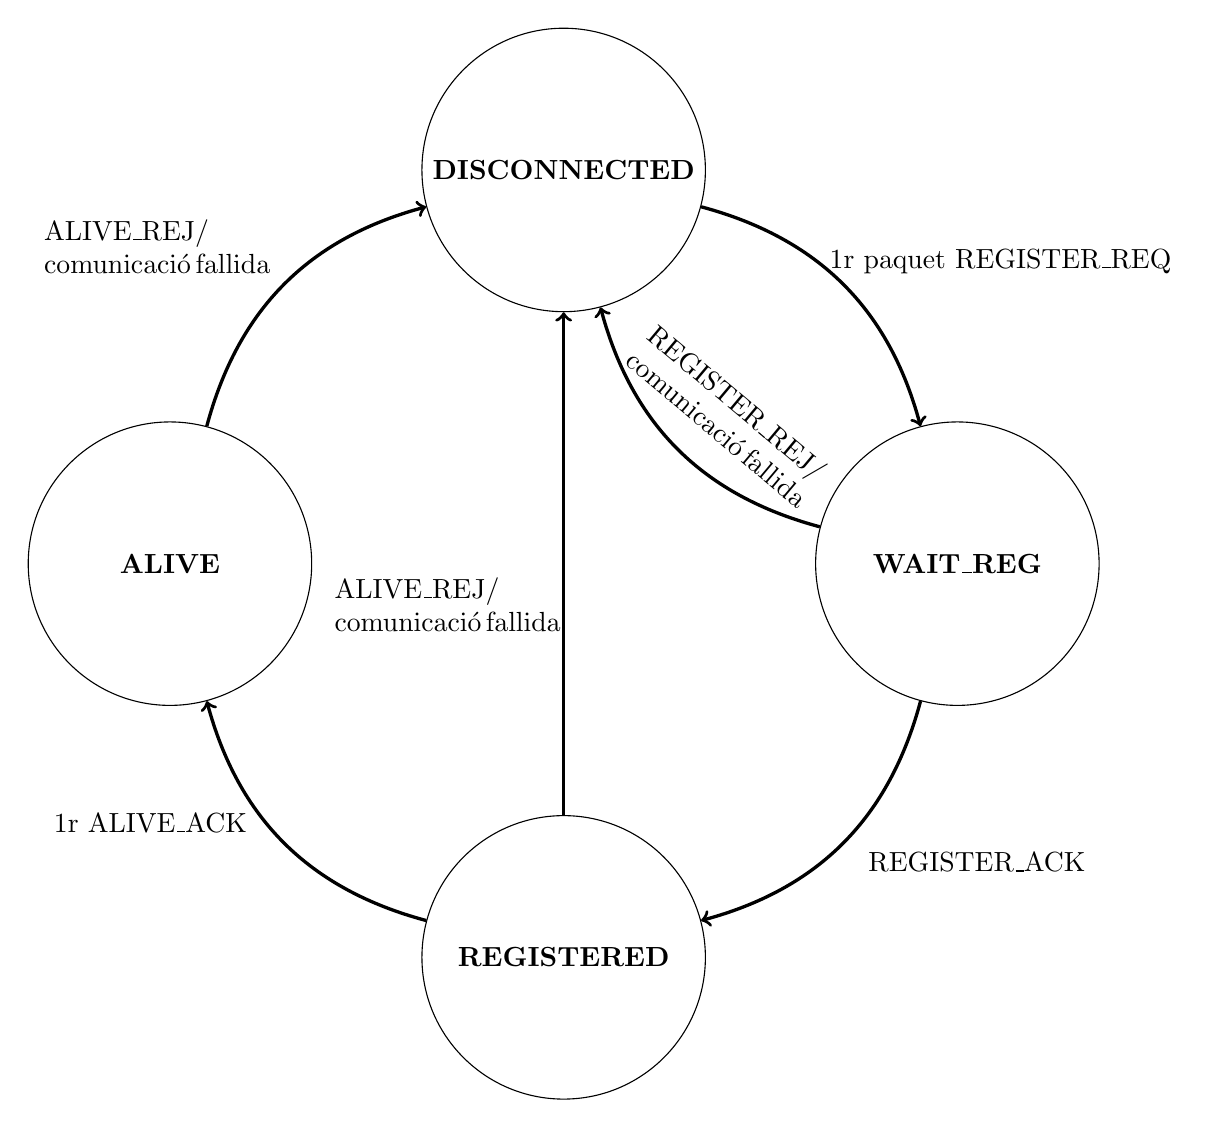
\begin{tikzpicture}

\tikzstyle{v} = [circle,minimum height = 36mm, draw=black]
\tikzstyle{e} = [->, very thick]

\node[v](D)at(5,5){\textbf{DISCONNECTED}};
\node[v](W)at(10,0){\textbf{WAIT\_REG}};
\node[v](R)at(5,-5){\textbf{REGISTERED}};
\node[v](A)at(0,0){\textbf{ALIVE}};


\draw[e](D) to [bend left,looseness=1] node[above, xshift=2cm] {1r paquet REGISTER\_REQ} (W);
\draw[e](W) to [bend left,looseness=1] node[above, yshift=0.5cm, xshift=-0.2cm, rotate= -40] {\parbox{1.5cm}{\centering REGISTER\_REJ/ \\ comunicació\,fallida} } (D);
\draw[e](R) to [bend left,looseness=1] node[above, xshift=-1.7cm] {1r ALIVE\_ACK} (A);
\draw[e](A) to [bend left,looseness=1] node[above, xshift=-2.3cm] {\parbox{1.5cm}{\centering ALIVE\_REJ/ \\ comunicació\,fallida} } (D);
\draw[e](W) to [bend left,looseness=1] node[above, xshift=1.7cm, yshift=-0.5cm] {REGISTER\_ACK} (R);
\draw[e](R) to  node[above, xshift=-2.16cm,yshift=-1cm] {\parbox{1.5cm}{\centering ALIVE\_REJ/ \\ comunicació\,fallida} } (D);

\end{tikzpicture}\\
\caption{Diagrama de la màquina d'estats del protocol implementat}
\end{figure}


\newpage
\section{Consideracions}
\subsection{Buffer consola}
La consola del client s'activa una vegada s'ha arribat a la fase d'alive. 
Si s'escriu alguna comanda quan això encara no ha passat, quan la consola
s'activi llegirà de l'entrada estàndard tot el que s'havia escrit quan aquesta
no estava activada. He pensat que deixar-ho així, o buidar el buffer de l'entrada
estàndard primer és una qüestió subjectiva més que un error ja que, per exemple,
si el client fa un quit per marxar, i la consola encara no està activada, el 
primer que farà quan s'activi és fer el quit. És per això que he decidit 
deixar-ho així.
\subsection{Llargada cua de clients}
A l'enunciat de la pràctica s'especifica que en les proves hi hauria 2 clients
de forma concurrent, així que s'ha triat de forma arbitrària que la cua 
de clients que el servidor és capaç d'escoltar és de 3 clients.
\subsection{SO\_REUSEADDR}
Fent una sèrie de tests al client, me'n vaig adonar que si s'utilitzava 
get-conf, es tancava el client i es tornava a executar amb inmediatesa 
saltava el següent error durant un petit termini de temps:
\begin{lstlisting}
[Errno 98] Address already in use
\end{lstlisting}

Pensant-me que era un error al meu codi a causa de un mal
tancament dels sockets, vaig cercar l'origen. Resulta ser que encara que
el socket es tanqui de forma correcta, el sistema operatiu té un temps
TIME\_WAIT abans que la stack de TCP consideri que la connexió ha estat
tancada completament. Aquest fet es pot evitar fàcilment amb l'opció
REUSEADDR:
\begin{lstlisting}
tcp_sock.setsockopt(socket.SOL_SOCKET, socket.SO_REUSEADDR, 1)
\end{lstlisting}

No obstant això, en ser una decisió del sistema operatiu, he considerat no
ficar-ho, i deixar que el meu programa sigui afectat per aquest temps
d'espera.

\subsection{Get-conf servidor de prova}
Una petita observació és que el servidor de proves penjat al campus virtual
envia dues vegades l'última línia de configuració quan se li demana amb
get-conf. Simplement a tenir en compte si s'utilitza per fer algun tipus
de test.









\end{document}
